\section{Introduction}
Increasingly, devices and services in our built environment are networked and can be controlled remotely. The proliferation of smart, controllable devices such as intelligent lighting, AV equipment, HVAC systems, or kitchen appliances raises the question of how to best interact with them. 

Today, commercial solutions use handheld mobile devices as {\em universal remote controls} to control such appliances. Commonly, users first browse a list of all available devices, and then call up a device-specific user interface. This method faces two challenges: {\em naming} and {\em scoping}. Assigning clear names is non-trivial. In shared spaces, the person trying to control the device might not be the one that named it - e.g., while an office building manager may know what ``Light 4 in area E'' corresponds to, an occupant may not. Second, without a method of scoping selection to automatically filter non-relevant devices, paging though long lists of names or navigating hierarchies becomes potentially more cumbersome than the physical action the ``convenient'' software solution was meant to replace.

To address these challenges, research has introduced techniques of augmenting mobile devices, e.g., with laser pointers, to enable direct aiming at target devices~\cite{beigl_point_1999,patel_2-way_2003}. While promising, some drawbacks of using handheld devices are that the device first has to be retrieved (e.g., from a pocket) and aimed; that two hands may be necessary for operation (one to hold the device, one to operate the touch screen); and that the user's visual attention is now split between looking down at a screen and out at the device to-be-controlled. 

\begin{figure}[t]
\centering
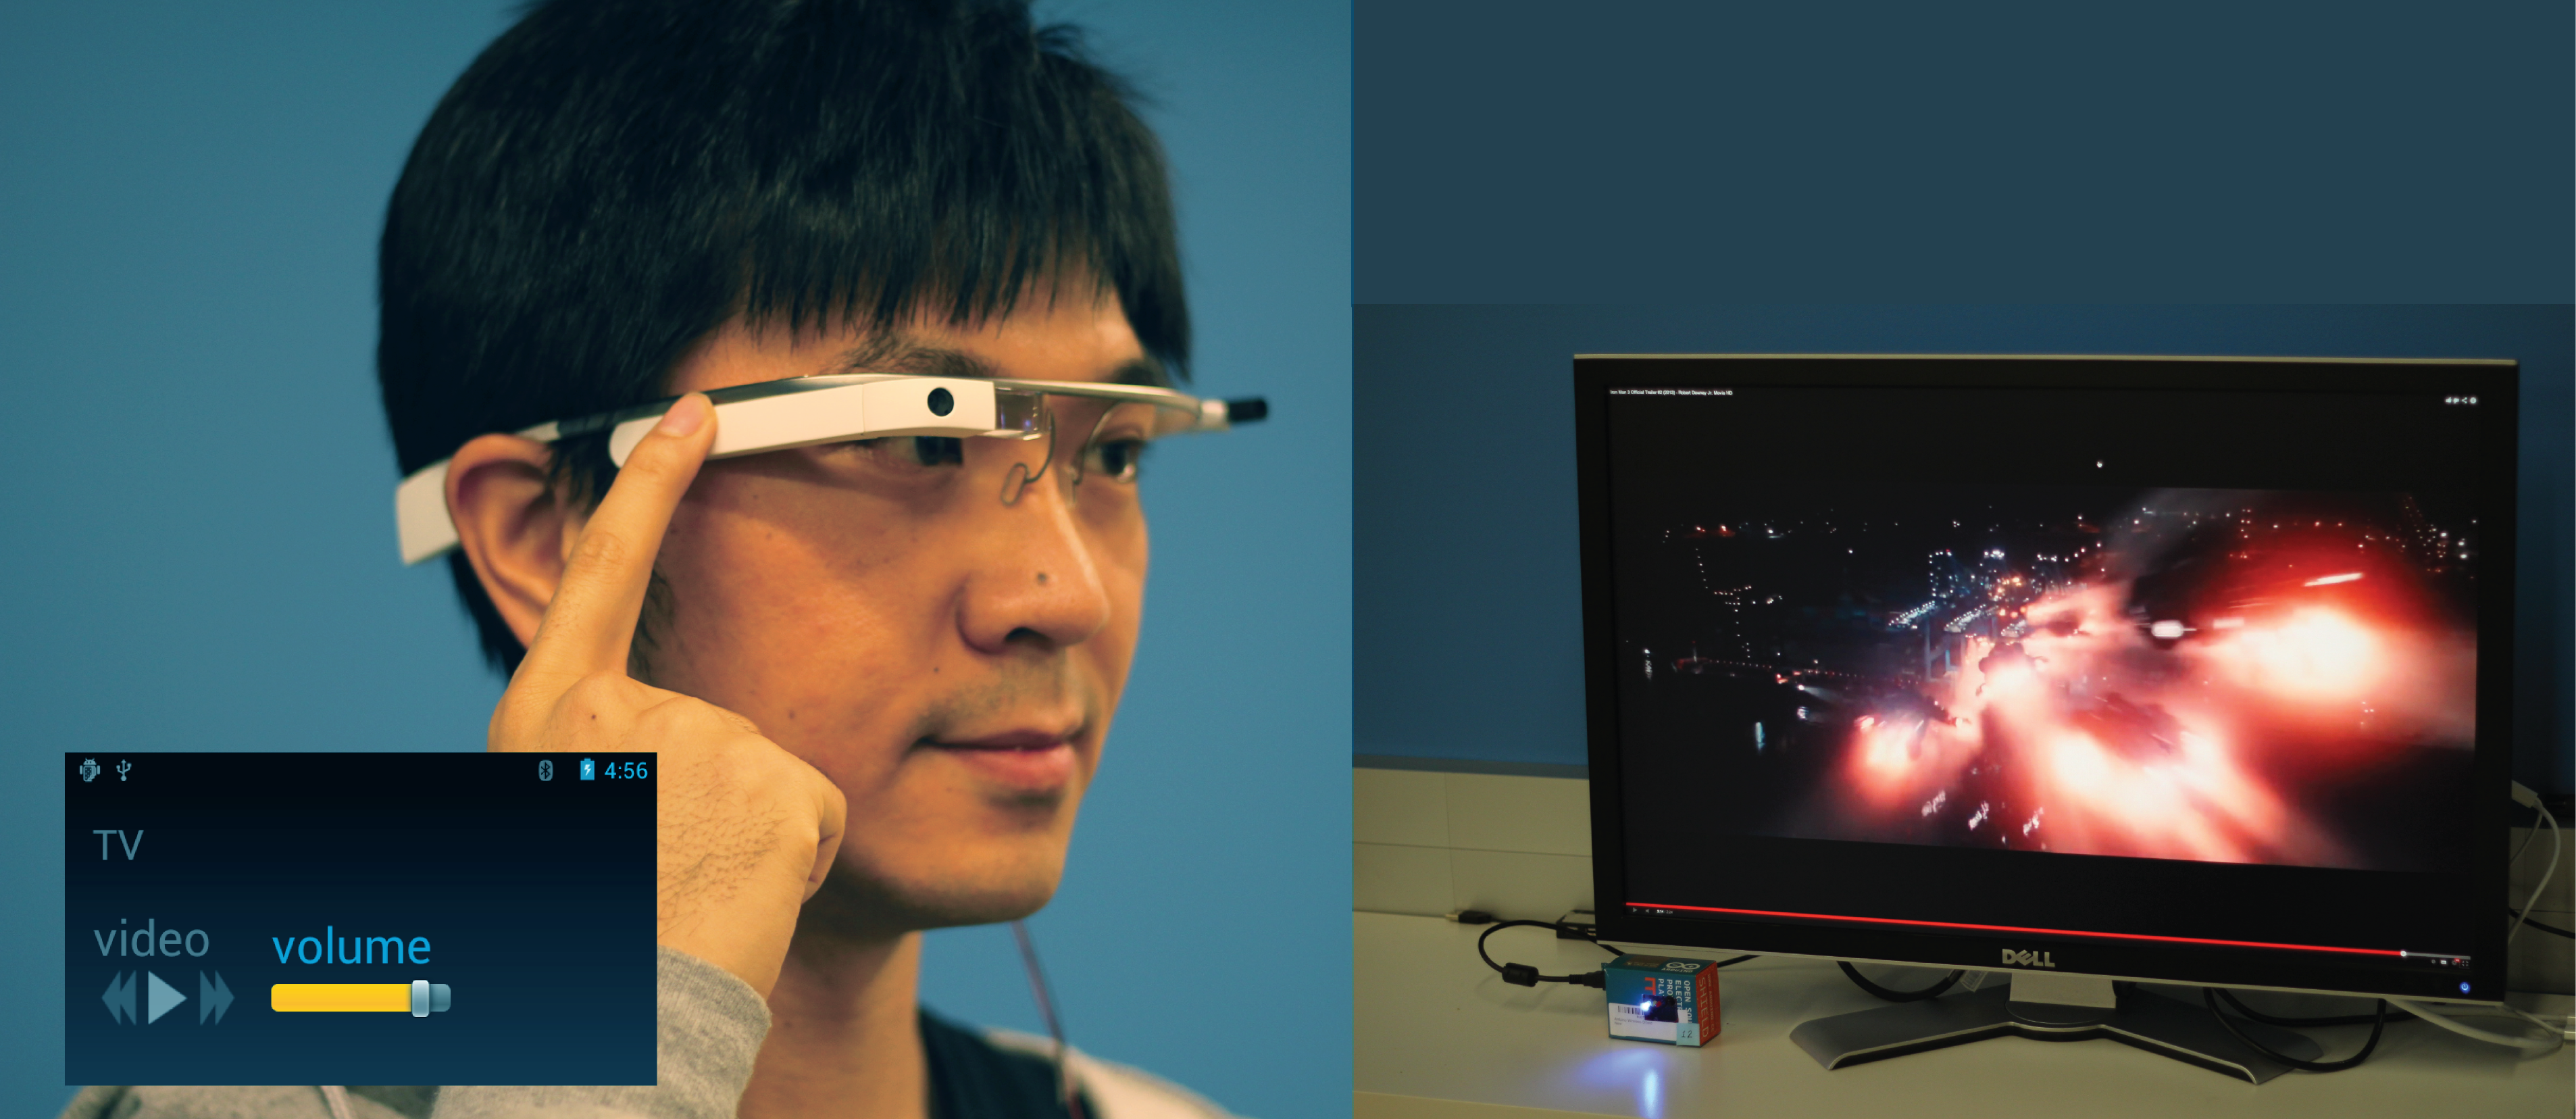
\includegraphics[width=1.0\columnwidth]{figures/teaser.jpg}
\caption{Using an augmented head-worn device (1), users can control smart home appliances (2) using head orientation targeting. A near-eye display (3) then shows an appliance control UI, which users navigate through multitouch gestures.}
\label{fig:teaser}
\end{figure}

In this paper, we introduce a novel method for selecting and controlling smart appliances in physical spaces through the use of a head-worn computing device with near-eye display and wireless communication. We augment Google Glass\footnote{\url{http://www.google.com/glass/start/}} with custom hardware for this purpose. Users first look in the direction of the device they wish to control to initiate interaction (e.g., at a lamp to control lighting, or at a speaker to change music playback volume).  If multiple devices fall within communication range, an disambiguation technique that combines on-screen information as well as visual feedback on the target devices lets users select their desired target. Once acquired, a device specific control UI shown on the head-mounted display enables adjustment of discrete and continuous parameters through a touchpad interface (see Figure~\ref{fig:teaser}).

Our hardware relies on infrared communication between Glass and target devices to establish a connection; and on wireless 802.15.4 radio communication to exchange control messages.  Glass is augmented with a narrow-beam IR emitter and a 802.15.4 radio. Target devices similarly have IR receivers and radios. This combination enables users to initiate interaction by orienting their head; but once initiated, users are free to look away from the target device while issuing control commands.

While prior work has tended to focus on proofs-of-concept, we also contribute empirical data on the system performance, usability, and user experience of  head-orientation targeting and device control. We first report measurements of range and beam characteristics of our controller. We then conduct a study with $15$ participants that compares acquisition times for physical targets in a room for our technique and an alternative list selection interface. We find that target acquisition through head orientation is preferred by users and is faster than list selection, given the constraints of linear input using a head-worn touch controller. We also report qualitative results from participants who use our system for home automation tasks.






